\begin{enunciado}{\ejExtra}
  En cierta especie animal se estudia la relación entre el peso $X$ (en kg) y el volumen pulmonar $Y$ (en litros), obteniéndose
  los datos:
  $$
    \begin{array}{|c||c|c|c|c|c|}
      \hline
      \text{peso (kg)}         & 60  & 85 & 100 & 150 & 250  \\ \hline
      \text{vol. pulmonar (l)} & 2.3 & 4  & 5   & 9   & 19.5 \\ \hline
    \end{array}
  $$
  \begin{enumerate}[label=(\alph*)]
    \item Ajustar los datos a una función $Y = a X^b$ en el sentido de cuadrados mínimos.
    \item En el procedimiento de mínimos cuadrados, hay una función que se minimiza, ¿Cuál es
          esa función y el valor del mínimo en este caso?
  \end{enumerate}
\end{enunciado}

\begin{enumerate}[label=(\alph*)]
  \item Primero hay que linealizar los parámetros del modelo, porque las ecuaciones normales que usamos para minimizar tienen que ser lineales:
        $$
          Y = a X^b
          \sii
          \ln(Y) = \ln(a X^b) =
          \ln(a) + \ln(X^b) =
          \ln(a) + b \cdot \ln(X)
        $$
        $$
          Y = a X^b
          \quad\taa{\red{!}}{}\equivalente\quad
          \tilde{Y}  = \tilde{a} + b \cdot \tilde{X}
        $$
        Armo sistema con los datos modificados después de la linealización:
        $$
          \llave{rcl}{
            0.83 & = & \tilde{a} + b \cdot 1.38 \\
            1.39 & = & \tilde{a} + b \cdot 4.44 \\
            1.61 & = & \tilde{a} + b \cdot 4.60 \\
            2.2  & = & \tilde{a} + b \cdot  5.01 \\
            2.97 & = & \tilde{a} + b \cdot 5.52
          }
          \flecha{forma}[matricial]
          A =
          \matriz{cc}{
            1 & 1.38 \\
            1 & 4.44 \\
            1 & 4.60 \\
            1 & 5.01 \\
            1 & 5.52
          }
          \matriz{c}{
            \tilde{a}\\
            b
          }
          =
          \matriz{c}{
            0.83 \\
            1.39 \\
            1.61 \\
            2.2 \\
            2.97
          }
        $$
        Armo ecuaciones normales y luego a resolver, rezando \orange{\faIcon{pray}}
        desde acá para que las cuentas no sean un infierno:
        {\tiny
        $$
          \begin{array}{rcl}
            A^tA\tilde{X} = A^t\tilde{Y}
                      & \sii                  &
            \matriz{ccccc}{
            1         & 1                     & 1    & 1    & 1    \\
            1.38      & 4.44                  & 4.60 & 5.01 & 5.52
            }
            \matriz{cc}{
            1         & 1.38                                       \\
            1         & 4.44                                       \\
            1         & 4.60                                       \\
            1         & 5.01                                       \\
            1         & 5.52
            }
            \matriz{c}{
            \tilde{a}                                              \\
              b
            }
            =
            \matriz{ccccc}{
            1         & 1                     & 1    & 1    & 1    \\
            1.38      & 4.44                  & 4.60 & 5.01 & 5.52
            }
            \matriz{c}{
            0.83                                                   \\
            1.39                                                   \\
            1.61                                                   \\
            2.2                                                    \\
              2.97
            }                                                      \\
                      & \Sii{\red{$\approx$}} &
            \matriz{cc}{
            5         & 21                                         \\
            21        & 98
            }
            \matriz{c}{
            \tilde{a}                                              \\
              \tilde{b}
            }
            =
            \matriz{c}{
            9                                                      \\
              42
            }                                                      \\
                      & \sii                  &
            \llave{rcl}{
            \tilde{a} & =                     & 0                  \\
            b         & =                     & 0.43
            }
          \end{array}
        $$
        }
        Queda demostrado que rezando las cuentas no son menos \textit{verga}. Tengo que volver a los parámetros del problema:
        $$
          a = e^0 = \blue{1}
          \ytext
          b = \blue{0.43}
          \Entonces{el modelo}[queda]
          \cajaResultado{
            Y = \blue{1} \cdot X^{\blue{0.43}}
          }
        $$
        Esto queda algo así
        $$
          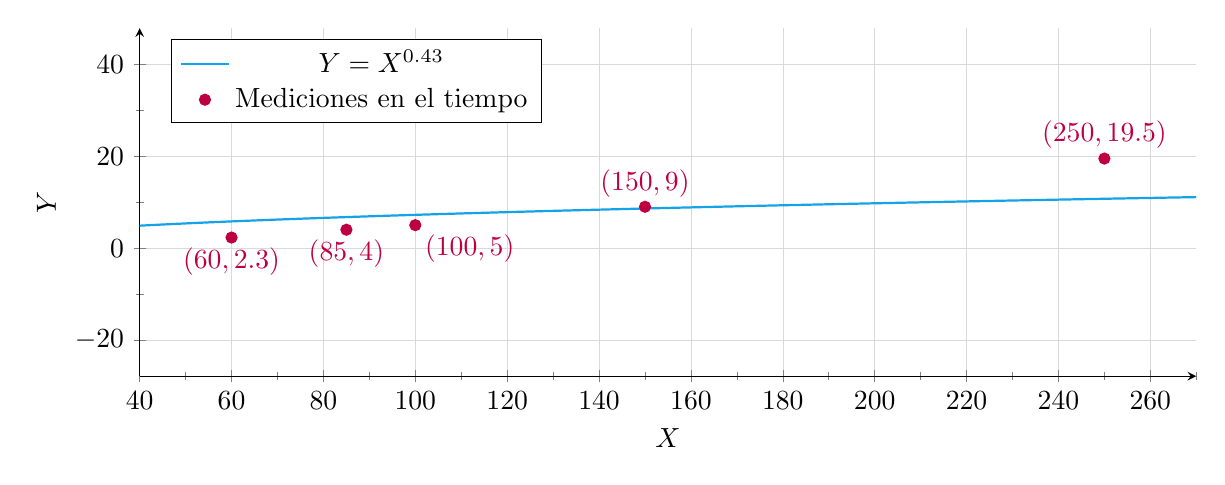
\begin{tikzpicture}
            \begin{axis}[
                axis lines = left,
                axis equal,
                xlabel = {$X$},
                ylabel = {$Y$},
                xmin = 40, xmax = 270,
                ymin = 0, ymax = 20,
                grid = major,
                grid style = {very thin, gray!30},
                minor tick num = 1,
                minor grid style = {very thin, gray!15},
                width = 15cm,
                height = 6cm,
                samples = 100,
                smooth,
                legend pos = north west
              ]

              \addplot[
                domain=30:270,
                Cerulean,
                thick
              ] {x^(0.43)};
              \addlegendentry{$Y = X^{0.43}$}

              \addplot[
                only marks,
                mark = *,
                mark size = 2pt,
                purple
              ] coordinates {
                  (60,2.3)
                  (85,4)
                  (100,5)
                  (150,9)
                  (250,19.5)
                };
              \addlegendentry{Mediciones en el tiempo}

              \node[below, purple] at (axis cs:60,2.3) {$(60,2.3)$};
              \node[below, purple] at (axis cs:85,4) {$(85,4)$};
              \node[below right, purple] at (axis cs:100,5) {$(100,5)$};
              \node[above, purple] at (axis cs:150,9) {$(150,9)$};
              \node[above, purple] at (axis cs:250,19.5) {$(250,19.5)$};

            \end{axis}
          \end{tikzpicture}
        $$

  \item La función a minimizar es la distancia de los valores de las mediciones a la función modelo:
        $$
          f(x_i, y_i) =
          \sumatoria{i = 1}{5} (Y_i - a X_i^b)^2 =
          \norma{\bm{Y} - a \bm{X}^b}_2^2
          \flecha{minimizar}[el sistema]
          \minimo\left(
          \norma{\bm{Y} - a \bm{X}^b}_2^2
          \right)
          \equivalente
          \minimo\left(
          \norma{\bm{\tilde{Y}} - \tilde{a} b\bm{\tilde{X}}}_2^2
          \right)
        $$
\end{enumerate}

\begin{aportes}
  \item \aporte{\dirRepo}{naD GarRaz \github}
\end{aportes}
